Having explored both Memcached and Redis, we now turn our attention to a `head to tail' comparison of the object caches. Initially, we focus on a comparison of the default performance. Subsequently, we expand the scope to multiple threads as well as multiple processes.


\section{Out of the Box}

Firstly, let us evaluate the default performance of Memcached and Redis (M\&R). The default performance is an important benchmark as well as a baseline. It is likely that M\&R users who simply require a cache which is `good' enough - performs to expectations, however, scalability is not a concern - will spend less time optimizing the cache performance and tuning the stack.

At this point, it is important to note that Memcached is a multi-threaded application with 4 threads by default. Figure \ref{fig:mr_default} plots M\&R performance with default configuration.

\begin{figure}[h]
    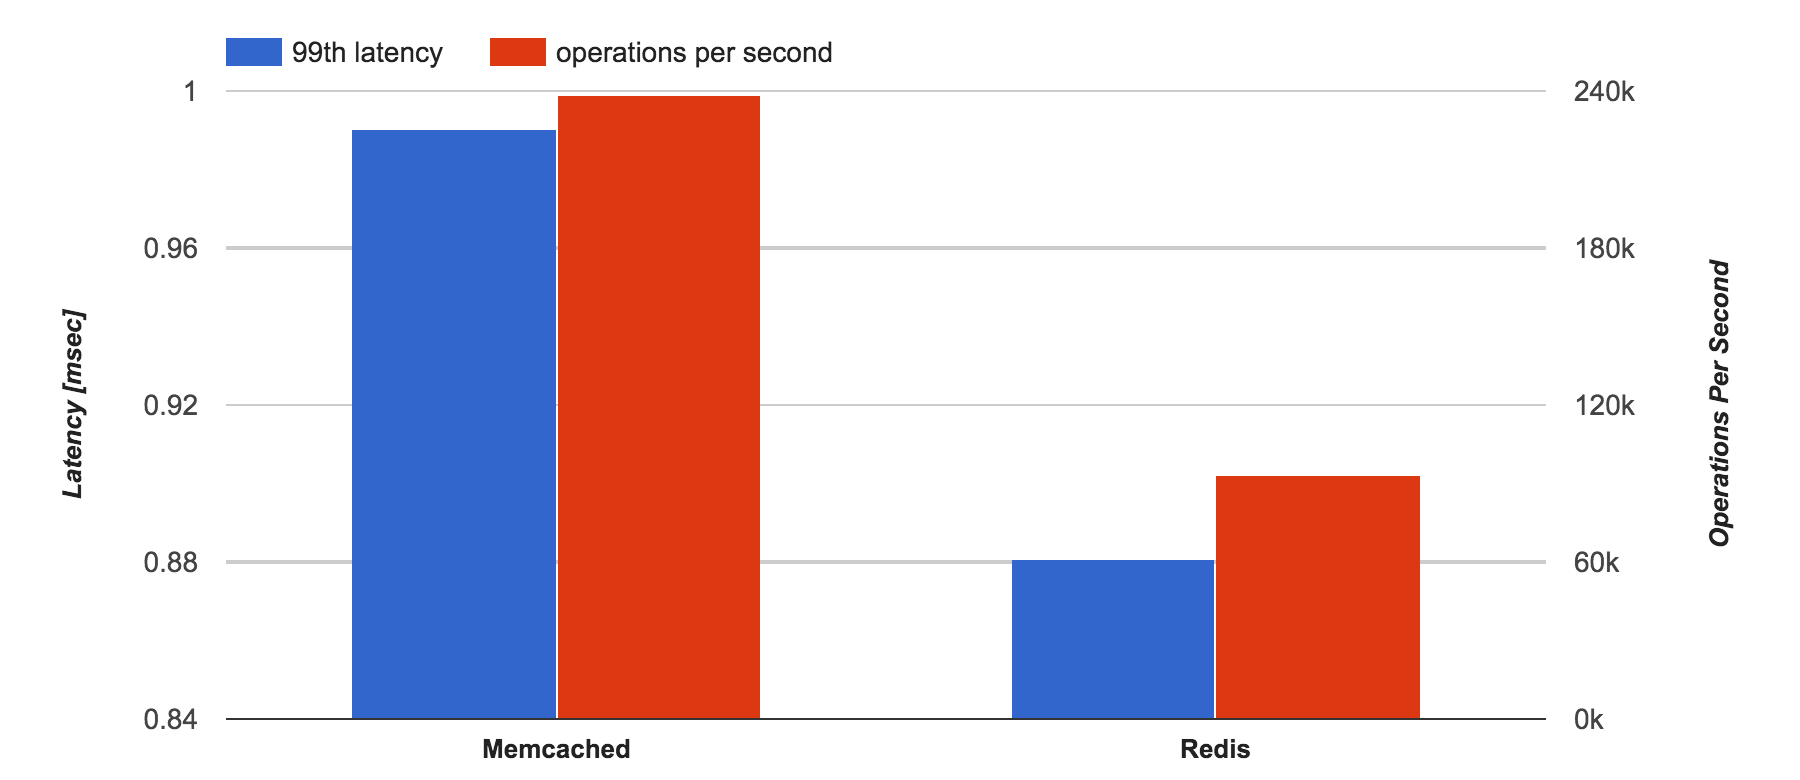
\includegraphics[width=\textwidth]{./res2/mr_default.png}
    \caption{Out of the Box config: 99th percentile latency \& Operations per second}
    \label{fig:mr_default}
\end{figure}

Memcached performs better in its default configuration. This is not an unsurprising result provided Memcached runs with 4 threads while Redis is single threaded. Interestingly, we would expect the performance of Memcached to be on the order of 4 times as much as Redis, however, Memcached only achieves close to 240k requests per second while Redis achieves 93k requests per second. This is about 2.5 times less than Memcached.

With default configuration, Memcached outperforms Redis. This is simply the result of utilizing 4 threads with Memcached. However, in the default configuration Memcached suffers from scalability inefficiencies. A comparison of a 4 threaded application vs a single threaded application may seem unfair, however, it is important to understand the baseline performance. In subsequent sections, we will focus on comparisons on a more even ground.

\section{Scaling up}
Let us now consider Memcached with multiple threads in comparison to multiple Redis instances.

\begin{figure}[h]
    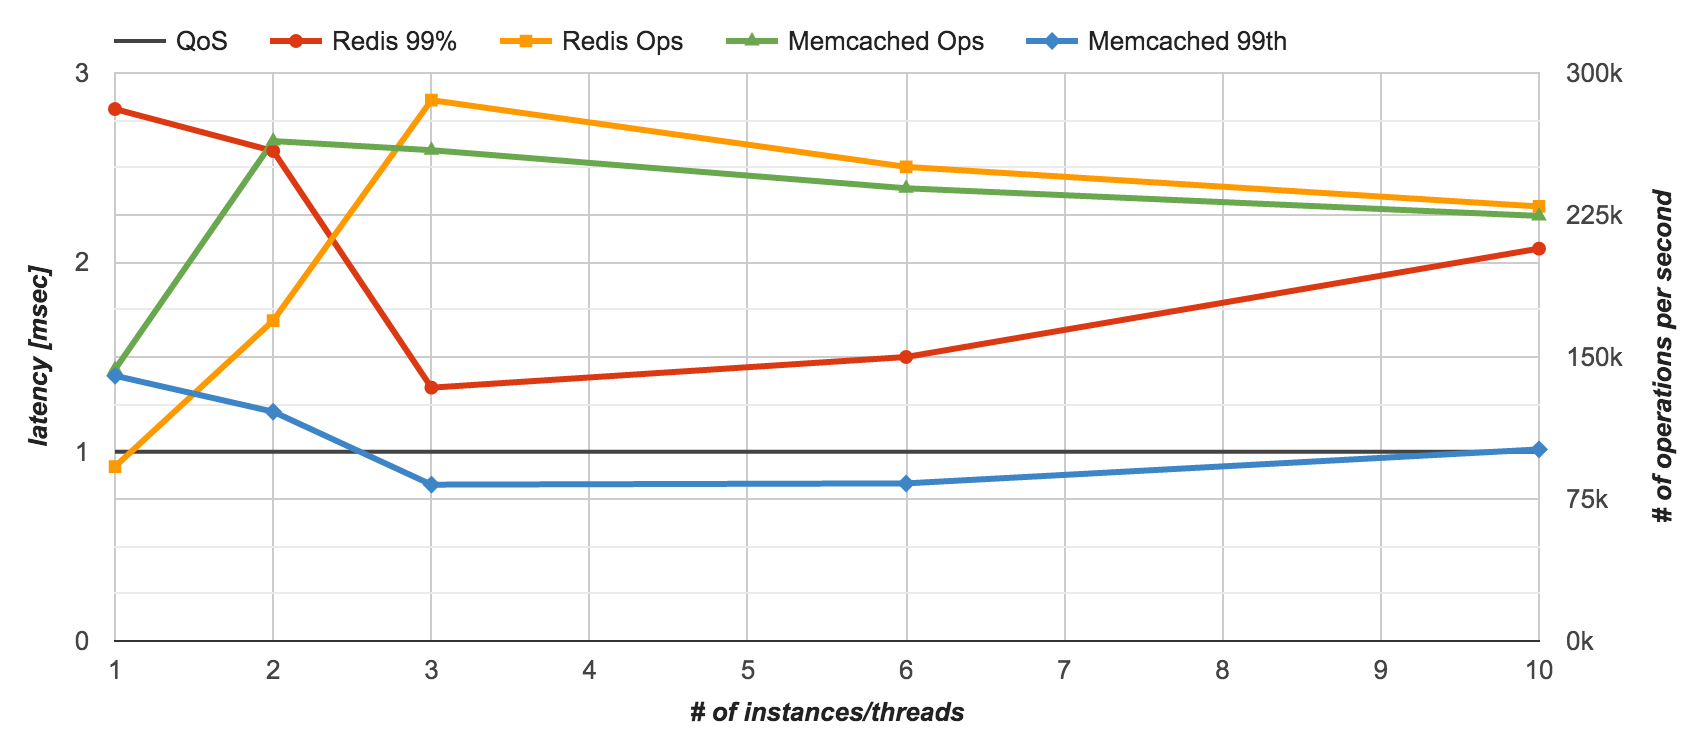
\includegraphics[width=\textwidth]{./res2/mr_instances.png}
    \caption{Memcached Threads vs Redis Instances: 99th percentile latency \& Operations per second}
    \label{fig:mr_instances}
\end{figure}
